\documentclass[10pt]{article}
\usepackage[usenames]{color} %used for font color
\usepackage{amssymb} %maths
\usepackage{amsmath} %maths
\usepackage[utf8]{inputenc} %useful to type directly diacritic characters
\usepackage{amsmath,amsthm,amssymb}
\usepackage{graphicx}
\usepackage{tikz}
\usetikzlibrary{arrows}
\usetikzlibrary{shapes.geometric}
\usepackage{centernot}
\tikzset{modal/.style={>=stealth',shorten >=1pt,auto, node distance=1.5cm, thick},
         world/.style={circle,draw,minimum size=1.5cm,fill= blue!10},
         worldr/.style={circle,draw,minimum size=1.5cm,fill=red!15},
         worldo/.style={circle,draw,minimum size=1.5cm,fill=orange!15},
         worldg/.style={circle,draw,minimum size=1.5cm ,fill=green!15},
         point/.style={circle,draw,inner sep=0.5mm,fill=black},
         n/.style={circle,draw=none,minimum size=1.6cm},
         n1/.style={draw=none},
         reflexive above/.style={->,loop,looseness=6,in=110,out=70},
         reflexive below/.style={->,loop,looseness=7,in=240,out=300},
         reflexive left/.style={->,loop,looseness=6,in=160 ,out=200},
         reflexive right/.style={->,loop,looseness=6,in=20,out=340}}              \begin{document}
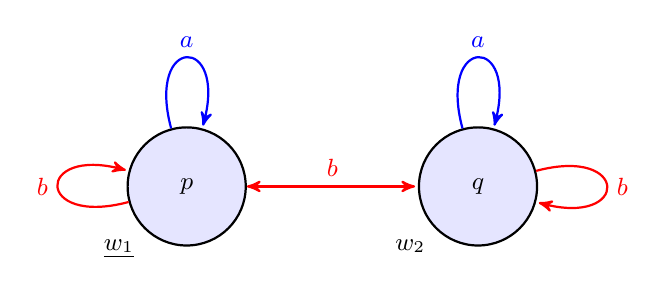
\begin{tikzpicture}[modal, node distance=3.7cm, font=\small]
\node[world] (1) [label= below left:{$\underline{w_1}$}]{$p$};
\node[world] (2) [right of=1] [label= below left:{$w_2$}]{$q$};
\path[<->](1) edge [red]          node {$b$} (2);  
\path[<->](1) edge [blue, loop above]  node {$a$} (1); 
\path[<->](2) edge [blue, loop above]  node {$a$} (2); 
\path[<->](1) edge [red, loop left]  node {$b$} (1);
\path[<->](2) edge [red, loop right]  node {$b$} (2); 
\end{tikzpicture}
\end{document}